\chapter{Benchmark \& Discussion}

In this chapter the three algorithms are benchmarked with different parameters and scenarios. The first series of tests is conducted in a static environment for a basic understanding of the algorithm performance and the second series is held in various dynamic settings to explore the dynamic capabilities of the algorithms. The testing environment was the minion cluster of the departement of informatics at the University of Zurich. The cluster consists of 16 machines and each machine has 128 GB RAM and two E5-2680 v2 at 2.80GHz processors. Every processor has 10 cores and the interlink between the machines is a 40Gbps Infiniband setup. The cluster has different partition speeds (slow, fast, superfast). All tests were conducted on superfast partitions.

\section{Results I: Algorithms Performance in Static Environments}

In this section, the static properties of the algorithms are going to be analysed and discussed.

\subsection{Solution Quality over Time}

The main focus of the work has been on the performance of the algorithms in terms of timeliness.  In this section, the three algorithms are going to be compared on their behaviour and the influence of the parameters density, number of agents and run mode (synchronous/asynchronous).

\begin{figure}[H]
\centering
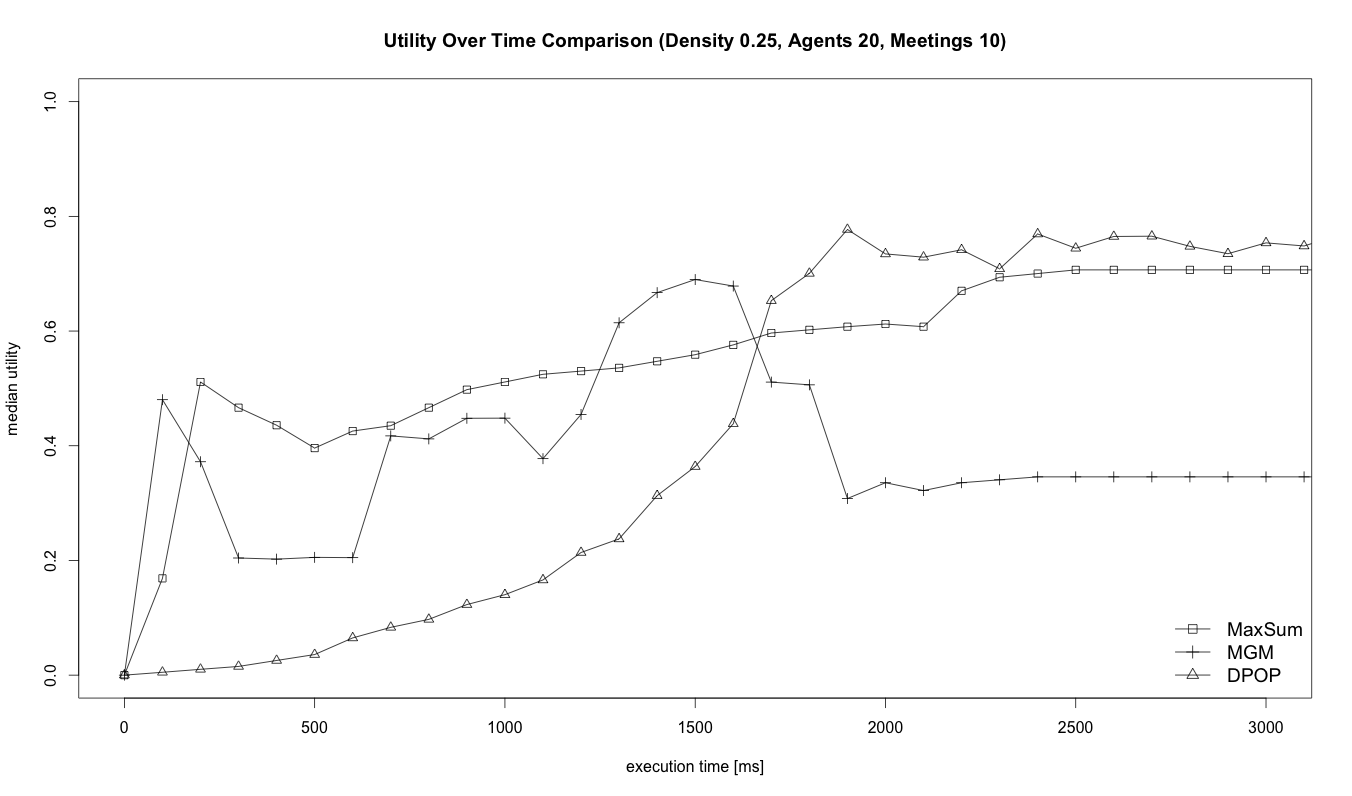
\includegraphics[width=430px]{graphics/experiments/static/quality/sq_1}
\caption{20/10, 0.25 density, all three, utility}
\label{fig:mgm_graph}
\end{figure}

\begin{figure}[H]
\centering
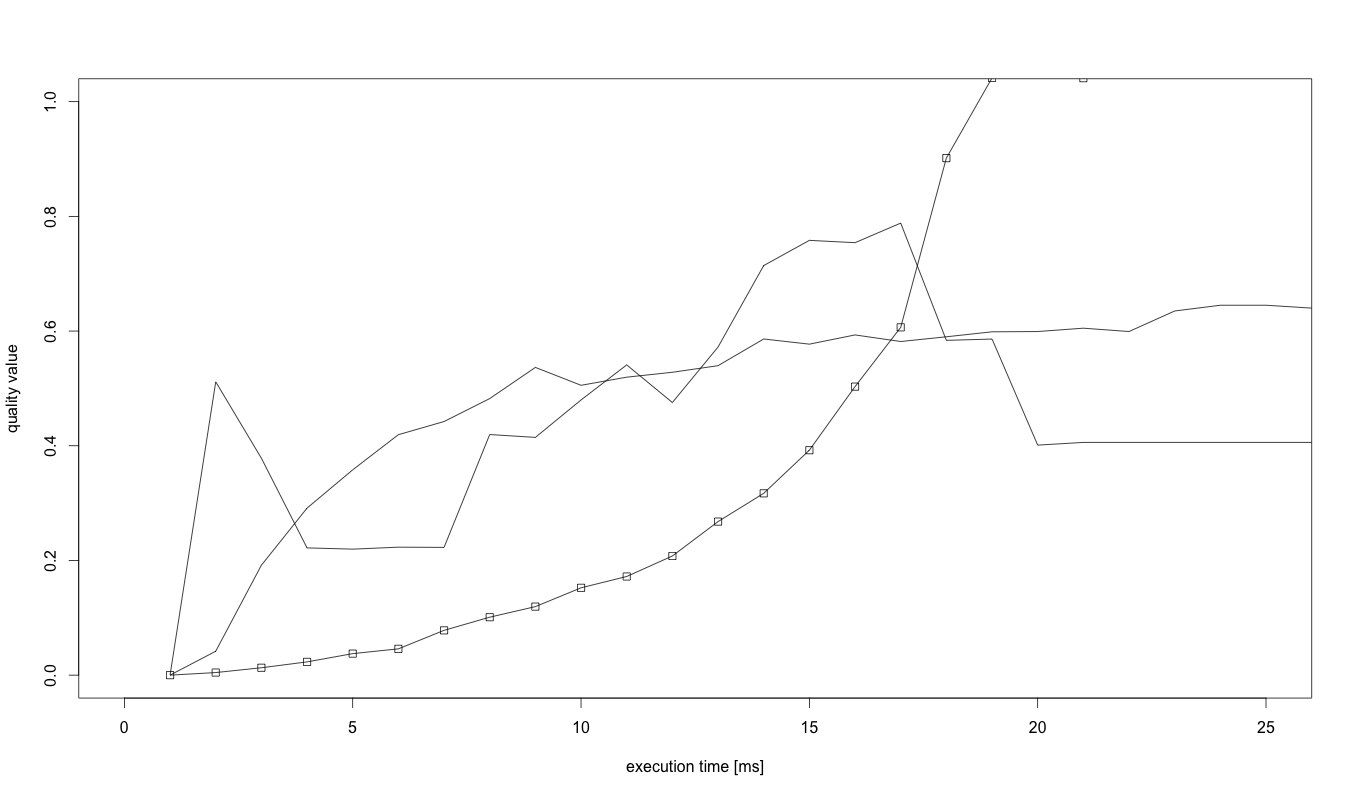
\includegraphics[width=430px]{graphics/experiments/static/quality/sq_2}
\caption{20/10, 0.25 density, all three, quality}
\label{fig:mgm_graph}
\end{figure}

%- Utility, Quality
%- Verlauf alle drei
%- Scalability: one, multiple machines
%- Quality Distribution

\subsection{Time to Convergence}

In this section, the time to convergence is going to be analyzed. The focus lays on the scalability properties of the algorithms in different densities and run modes (synchronous/asynchronous) in regards to agents. Meetings have, because of the participation limitation a limited influence on the performance of the algorithms when meeting numbers are increased. 

%\begin{tabular}{llr}
%\toprule
%\multicolumn{2}{c}{Meetings Scalability (Asynchronous) \\
%\cmidrule(r){1-4}
%Meetings & MaxSum   & MGM & DPOP \\
%\midrule
%10 &        244.3     & 10.3 &	77.8\\
%20  &     91.8	     & 4.4 & 63.7\\
%30 &     70.7       	& 2.6 & 67.7\\
%40 &     26.7     & 2.4 & 71\\
%50 &     31.5     &	2.3 & 45\\
%
%\bottomrule
%\end{tabular}
%
%\begin{tabular}{llr}
%\toprule
%\multicolumn{2}{c}{Meetings Scalability (Synchronous) \\
%\cmidrule(r){1-4}
%Meetings & MaxSum   & MGM & DPOP \\
%\midrule
%10 & 31.1	 & 46.45 &	100.2\\
%20  & 6.75	 & 38.7 & 91.5\\
%30 & 2.6	& 33.8 & 63.25\\
%40 & 2.3 & 34.65 & 57.85\\
%50 & 2.3 & 23.95 &	67.3\\
%
%\bottomrule
%\end{tabular}

%- More time to find a valid solution -> could be local optima
%- Scalability: one, multiple machines
%- Convergence Distribution: how often does it converge -> dpop should always converge
%

\section{Results II: Algorithms Performance in Dynamic Environments}

In the Results II section, the dynamic abilities of the algorithms are going to be tested. Two evaluation values have been chosen. The value for stability has been chosen to be rate / avg. utility comparable to  \cite{Mailler2014}. Instead of using the conflicts, it was decided to use the utility value. Rate is defined as dP/dt, whereas dP is the amount of change to constraints. It was modelled to use different amounts of change. For the rebound time it was chosen to use difference between the utility at the timepoint one step after the change and the next change interval time step. Formally, Bounceback b -> \(u(t_{cj})-u(t_{c_i+1}\)

\subsection{Quality Stability}







\subsection{Average Rebound}



